\documentclass[aspectratio=169]{beamer}

\usepackage[T2A]{fontenc}
\usepackage[utf8]{inputenc}
\usepackage[russian,english]{babel}
\usepackage{graphics}
%\usepackage[normalem]{ulem}

\graphicspath{{res/}}
\DeclareGraphicsExtensions{.png,.jpg}

\usetheme{Copenhagen}

\title{Текстовый редактор Vim}
\author{Чубий Савва}
\institute{Лицей НИУ ВШЭ}
\date{}%TODO

\begin{document}
    \begin{frame}
        \maketitle
    \end{frame}

    \begin{frame}\frametitle{Что такое vim? Основные моменты.}
        \begin{columns}[T,onlytextwidth]
            \begin{column}{0.6\textwidth}
                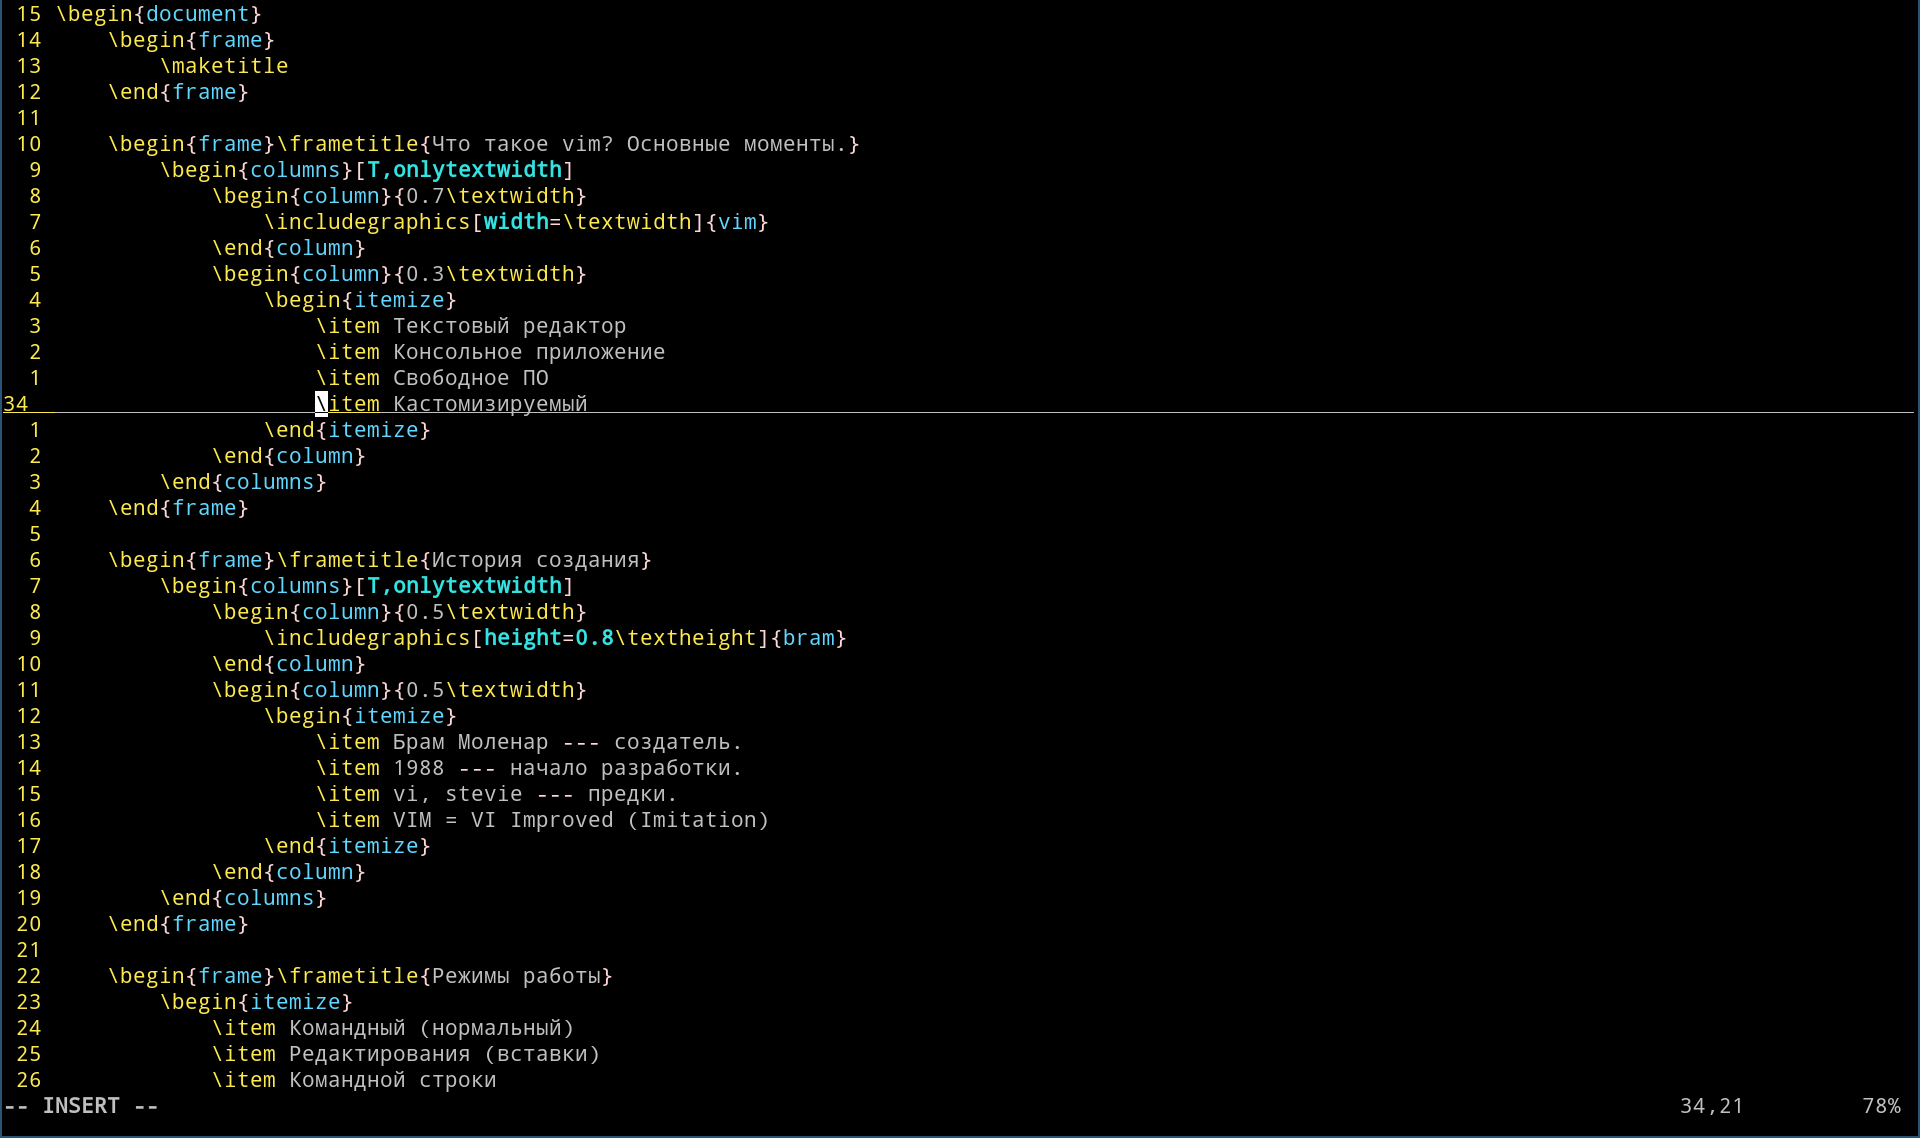
\includegraphics[width=\textwidth]{vim}
            \end{column}
            \begin{column}{0.4\textwidth}
                \begin{itemize}
                    \item Текстовый редактор
                    \item Консольное приложение (изначально)
                    \item Легкий
                    \item Свободное ПО
                    \item Кастомизируемый
                    \item "Мини IDE"
                    \item Установлен на большинстве компьютеров под linux
                    \item Есть версии под многие платформы
                \end{itemize}
            \end{column}
        \end{columns}
    \end{frame}

    \begin{frame}\frametitle{История создания}
        \begin{columns}[T,onlytextwidth]
            \begin{column}{0.5\textwidth}
                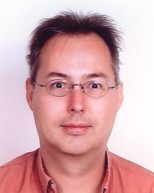
\includegraphics[height=0.8\textheight]{bram}
            \end{column}
            \begin{column}{0.5\textwidth}
                \begin{itemize}
                    \item Брам Моленар --- создатель.
                    \item 1988 --- начало разработки.
                    \item vi, stevie --- предки.
                    \item VIM = VI IMproved (IMitation)
                \end{itemize}
            \end{column}
        \end{columns}
    \end{frame}

    \begin{frame}\frametitle{Части интерфейса}
        \begin{columns}[T,onlytextwidth]
            \begin{column}{0.7\textwidth}
                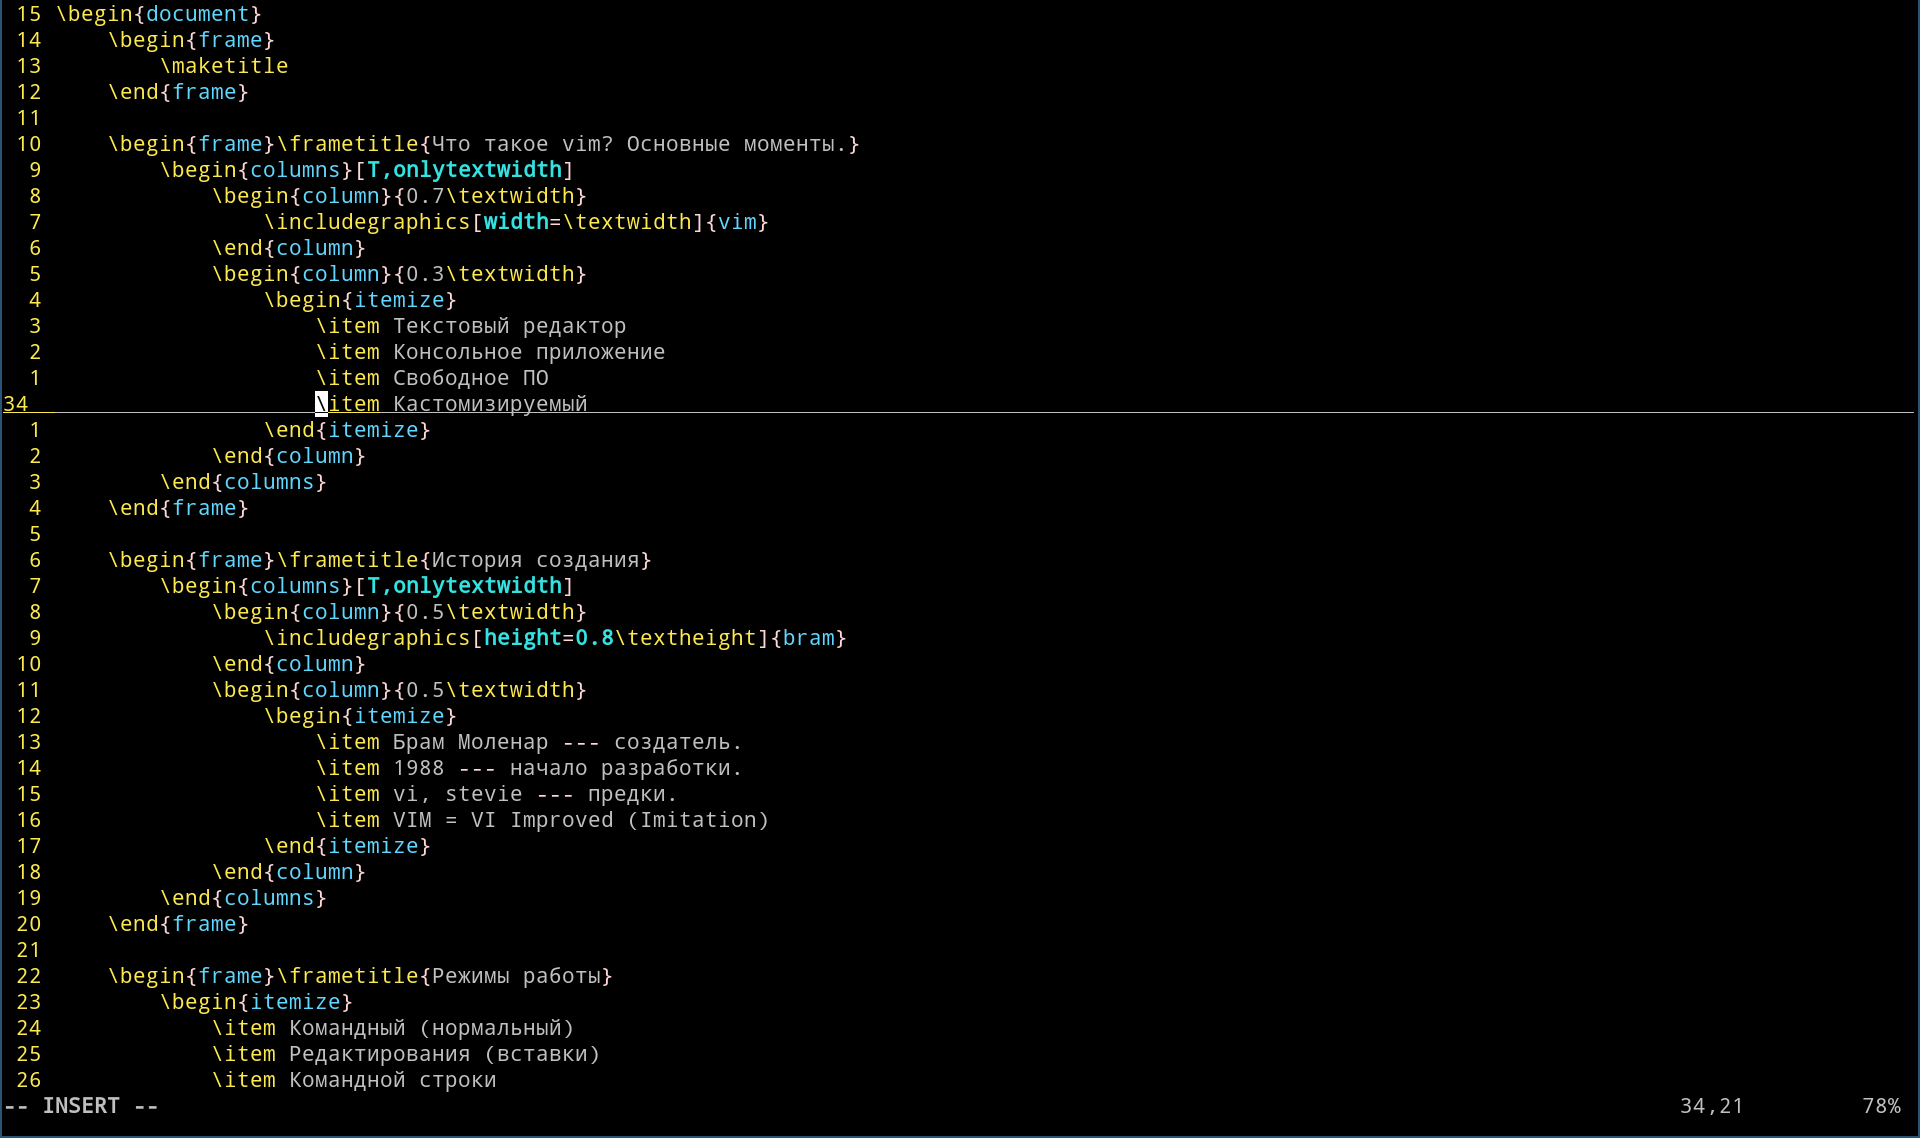
\includegraphics[width=\textwidth]{vim}
            \end{column}
            \begin{column}{0.3\textwidth}
                \begin{itemize}
                    \item Основная часть
                    \item Номера строк
                    \item Строка состояния
                \end{itemize}
            \end{column}
        \end{columns}
    \end{frame}

    \begin{frame}\frametitle{Режимы работы}
        \begin{itemize}
            \item Командный (нормальный)
            \item Редактирования (вставки)
            \item Командной строки
            \item Выделения (визуальный)
        \end{itemize}
    \end{frame}

    \begin{frame}\frametitle{Командный (нормальный) режим}
        \begin{itemize}
            \item Команда --- сочетание клавиш
            \begin{itemize}
                \item Перемещение --- $h, j, k, l$
                \item Заменить символ --- $r$
                \item Вырезать строку --- $dd$
                \item Вырезать 10 строк --- $d10j$
                \item Вставить --- $p$
            \end{itemize}
            \item Переход в другие режимы
            \begin{itemize}
                \item Редактирование --- $i, I, a, A, o, O, r, R$
                \item Командной строки --- $:$
                \item Выделения --- $v, C-v, V$
            \end{itemize}
            \item Возвращение из др. режимов --- $Esc$
        \end{itemize}
    \end{frame}

    \begin{frame}\frametitle{Режим редактирования (вставки)}
        \begin{itemize}
            \item Обычное редактирование текста
            \item Перемещение только $\leftarrow, \downarrow, \downarrow, \rightarrow$
            \item Сочетания клавиш с $C-$
        \end{itemize}
    \end{frame}

    \begin{frame}\frametitle{Режим выделения (визуальный)}
        \begin{columns}[T,onlytextwidth]
            \begin{column}{0.5\textwidth}
                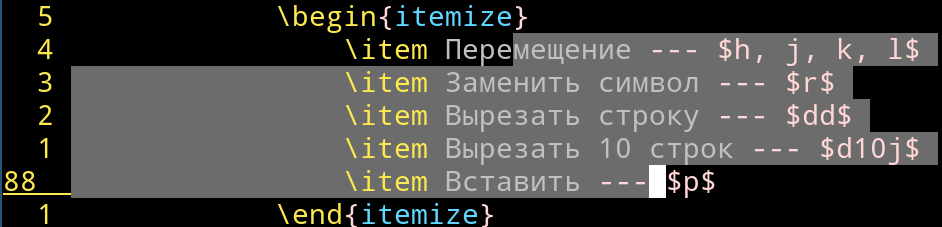
\includegraphics[width=\textwidth]{visual_v}\\~\\
                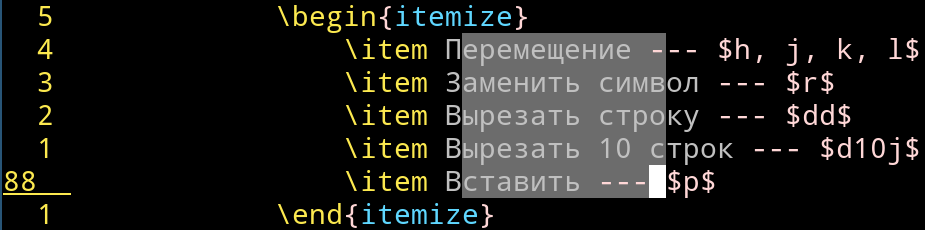
\includegraphics[width=\textwidth]{visual_C-v}\\~\\
                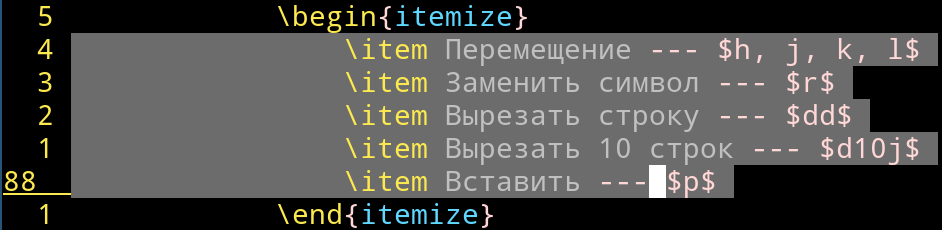
\includegraphics[width=\textwidth]{visual_V}\\~\\
            \end{column}
            \begin{column}{0.5\textwidth}
                \begin{itemize}
                    \item Обычное выделение --- $v$\\
                    \item Выделение блока --- $C-v$\\
                    \item Выделение строк --- $V$\\
                \end{itemize}
            \end{column}
        \end{columns}
    \end{frame}

    \begin{frame}\frametitle{Режим командной строки}
        \begin{itemize}
            \item $:$ перед командой
            \item Выполнение обычных команд --- $!$\\
                Например, $:!python3\ main.py$
            \item Сохранение --- $:w$
            \item Выход --- $:q$
            \item Выход с сохранением --- $:wq$
            \item Замена в тексте --- $\%s/old/new/g$
            \item Временные настройки
        \end{itemize}
    \end{frame}

    \begin{frame}\frametitle{Файл конфигурации $\sim/.vimrc$}
        \begin{columns}[T,onlytextwidth]
            \begin{column}{0.24\textwidth}
                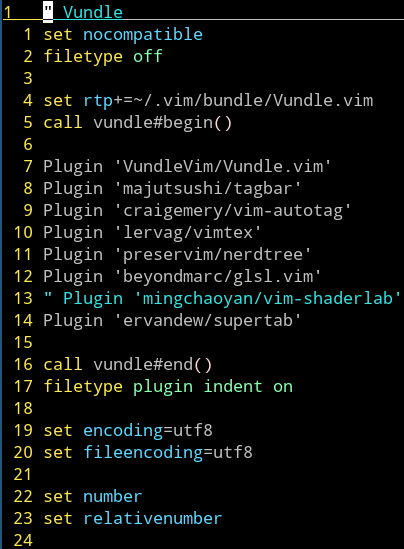
\includegraphics[width=\textwidth]{vimrc1}
            \end{column}
            \begin{column}{0.24\textwidth}
                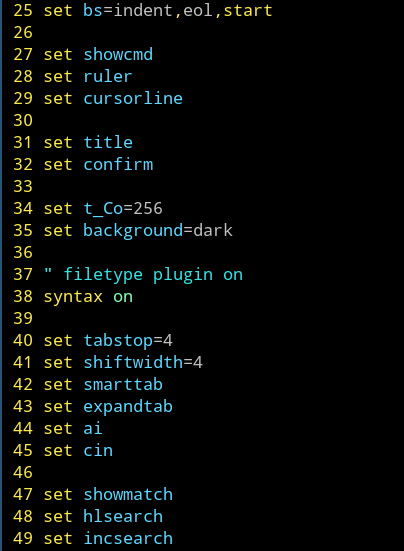
\includegraphics[width=\textwidth]{vimrc2}
            \end{column}
            \begin{column}{0.5\textwidth}
                \begin{itemize}
                    \item Плагины
                    \item Скрипты
                    \item Постоянные настройки
                    \item Макросы
                \end{itemize}
            \end{column}
        \end{columns}
    \end{frame}

    \begin{frame}\frametitle{Другие возможности}
        \begin{itemize}
            \item Поиск в тексте
            \item Code folding
            \item Code highliting
            \item Вкладки
            \item Разделение окна на несколько частей
            \item Как файловый менеджер
            \item Сохранение истории изменения файла
            \item Встроенная справка
            \item Автодополнение
            \item Проверка правописания
            \item \textit{Подключение по ftp}
        \end{itemize}
    \end{frame}
\end{document}
